% Options for packages loaded elsewhere
\PassOptionsToPackage{unicode}{hyperref}
\PassOptionsToPackage{hyphens}{url}
%
\documentclass[
]{article}
\usepackage{amsmath,amssymb}
\usepackage{lmodern}
\usepackage{iftex}
\ifPDFTeX
  \usepackage[T1]{fontenc}
  \usepackage[utf8]{inputenc}
  \usepackage{textcomp} % provide euro and other symbols
\else % if luatex or xetex
  \usepackage{unicode-math}
  \defaultfontfeatures{Scale=MatchLowercase}
  \defaultfontfeatures[\rmfamily]{Ligatures=TeX,Scale=1}
\fi
% Use upquote if available, for straight quotes in verbatim environments
\IfFileExists{upquote.sty}{\usepackage{upquote}}{}
\IfFileExists{microtype.sty}{% use microtype if available
  \usepackage[]{microtype}
  \UseMicrotypeSet[protrusion]{basicmath} % disable protrusion for tt fonts
}{}
\makeatletter
\@ifundefined{KOMAClassName}{% if non-KOMA class
  \IfFileExists{parskip.sty}{%
    \usepackage{parskip}
  }{% else
    \setlength{\parindent}{0pt}
    \setlength{\parskip}{6pt plus 2pt minus 1pt}}
}{% if KOMA class
  \KOMAoptions{parskip=half}}
\makeatother
\usepackage{xcolor}
\IfFileExists{xurl.sty}{\usepackage{xurl}}{} % add URL line breaks if available
\IfFileExists{bookmark.sty}{\usepackage{bookmark}}{\usepackage{hyperref}}
\hypersetup{
  pdftitle={Getting-Started},
  pdfauthor={Diana Nurbakova},
  hidelinks,
  pdfcreator={LaTeX via pandoc}}
\urlstyle{same} % disable monospaced font for URLs
\usepackage[margin=1in]{geometry}
\usepackage{color}
\usepackage{fancyvrb}
\newcommand{\VerbBar}{|}
\newcommand{\VERB}{\Verb[commandchars=\\\{\}]}
\DefineVerbatimEnvironment{Highlighting}{Verbatim}{commandchars=\\\{\}}
% Add ',fontsize=\small' for more characters per line
\usepackage{framed}
\definecolor{shadecolor}{RGB}{248,248,248}
\newenvironment{Shaded}{\begin{snugshade}}{\end{snugshade}}
\newcommand{\AlertTok}[1]{\textcolor[rgb]{0.94,0.16,0.16}{#1}}
\newcommand{\AnnotationTok}[1]{\textcolor[rgb]{0.56,0.35,0.01}{\textbf{\textit{#1}}}}
\newcommand{\AttributeTok}[1]{\textcolor[rgb]{0.77,0.63,0.00}{#1}}
\newcommand{\BaseNTok}[1]{\textcolor[rgb]{0.00,0.00,0.81}{#1}}
\newcommand{\BuiltInTok}[1]{#1}
\newcommand{\CharTok}[1]{\textcolor[rgb]{0.31,0.60,0.02}{#1}}
\newcommand{\CommentTok}[1]{\textcolor[rgb]{0.56,0.35,0.01}{\textit{#1}}}
\newcommand{\CommentVarTok}[1]{\textcolor[rgb]{0.56,0.35,0.01}{\textbf{\textit{#1}}}}
\newcommand{\ConstantTok}[1]{\textcolor[rgb]{0.00,0.00,0.00}{#1}}
\newcommand{\ControlFlowTok}[1]{\textcolor[rgb]{0.13,0.29,0.53}{\textbf{#1}}}
\newcommand{\DataTypeTok}[1]{\textcolor[rgb]{0.13,0.29,0.53}{#1}}
\newcommand{\DecValTok}[1]{\textcolor[rgb]{0.00,0.00,0.81}{#1}}
\newcommand{\DocumentationTok}[1]{\textcolor[rgb]{0.56,0.35,0.01}{\textbf{\textit{#1}}}}
\newcommand{\ErrorTok}[1]{\textcolor[rgb]{0.64,0.00,0.00}{\textbf{#1}}}
\newcommand{\ExtensionTok}[1]{#1}
\newcommand{\FloatTok}[1]{\textcolor[rgb]{0.00,0.00,0.81}{#1}}
\newcommand{\FunctionTok}[1]{\textcolor[rgb]{0.00,0.00,0.00}{#1}}
\newcommand{\ImportTok}[1]{#1}
\newcommand{\InformationTok}[1]{\textcolor[rgb]{0.56,0.35,0.01}{\textbf{\textit{#1}}}}
\newcommand{\KeywordTok}[1]{\textcolor[rgb]{0.13,0.29,0.53}{\textbf{#1}}}
\newcommand{\NormalTok}[1]{#1}
\newcommand{\OperatorTok}[1]{\textcolor[rgb]{0.81,0.36,0.00}{\textbf{#1}}}
\newcommand{\OtherTok}[1]{\textcolor[rgb]{0.56,0.35,0.01}{#1}}
\newcommand{\PreprocessorTok}[1]{\textcolor[rgb]{0.56,0.35,0.01}{\textit{#1}}}
\newcommand{\RegionMarkerTok}[1]{#1}
\newcommand{\SpecialCharTok}[1]{\textcolor[rgb]{0.00,0.00,0.00}{#1}}
\newcommand{\SpecialStringTok}[1]{\textcolor[rgb]{0.31,0.60,0.02}{#1}}
\newcommand{\StringTok}[1]{\textcolor[rgb]{0.31,0.60,0.02}{#1}}
\newcommand{\VariableTok}[1]{\textcolor[rgb]{0.00,0.00,0.00}{#1}}
\newcommand{\VerbatimStringTok}[1]{\textcolor[rgb]{0.31,0.60,0.02}{#1}}
\newcommand{\WarningTok}[1]{\textcolor[rgb]{0.56,0.35,0.01}{\textbf{\textit{#1}}}}
\usepackage{graphicx}
\makeatletter
\def\maxwidth{\ifdim\Gin@nat@width>\linewidth\linewidth\else\Gin@nat@width\fi}
\def\maxheight{\ifdim\Gin@nat@height>\textheight\textheight\else\Gin@nat@height\fi}
\makeatother
% Scale images if necessary, so that they will not overflow the page
% margins by default, and it is still possible to overwrite the defaults
% using explicit options in \includegraphics[width, height, ...]{}
\setkeys{Gin}{width=\maxwidth,height=\maxheight,keepaspectratio}
% Set default figure placement to htbp
\makeatletter
\def\fps@figure{htbp}
\makeatother
\setlength{\emergencystretch}{3em} % prevent overfull lines
\providecommand{\tightlist}{%
  \setlength{\itemsep}{0pt}\setlength{\parskip}{0pt}}
\setcounter{secnumdepth}{-\maxdimen} % remove section numbering
\ifLuaTeX
  \usepackage{selnolig}  % disable illegal ligatures
\fi

\title{Getting-Started}
\author{Diana Nurbakova}
\date{2022-03-06}

\begin{document}
\maketitle

\hypertarget{initialisation}{%
\subsection{Initialisation}\label{initialisation}}

Créer un projet \texttt{R} :

\texttt{File} -\textgreater{} \texttt{New\ Project...} -\textgreater{}
\texttt{New\ Directory}

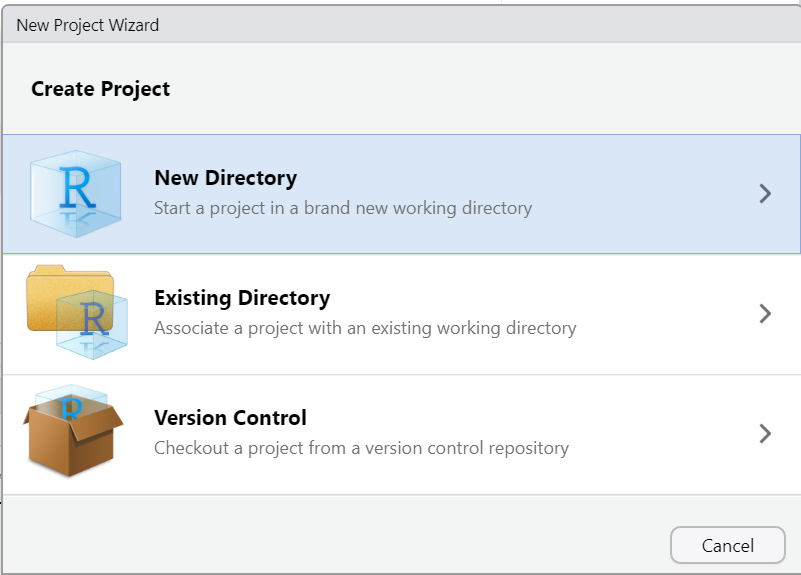
\includegraphics[width=0.5\textwidth,height=\textheight]{img/init-new-dir.png}

-\textgreater{} \texttt{New\ Directory} -\textgreater{}
\texttt{New\ Project} (type du projet)

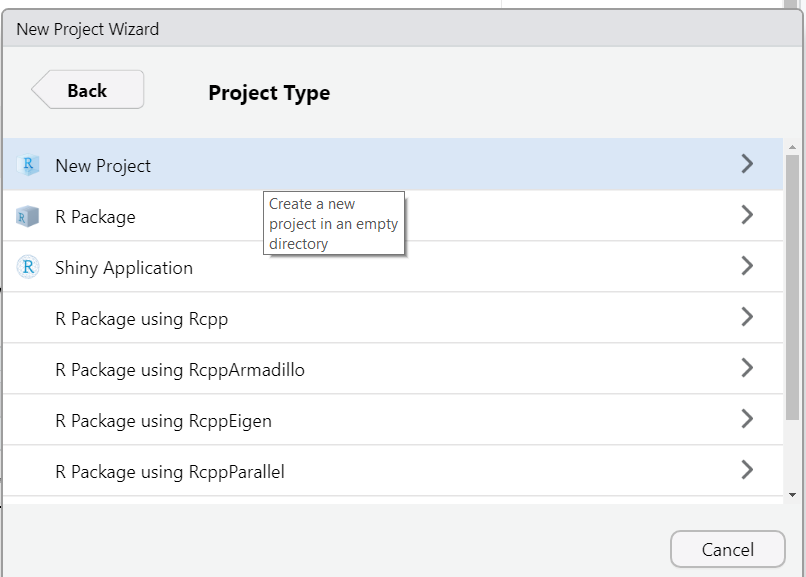
\includegraphics[width=0.5\textwidth,height=\textheight]{img/init-new-project.png}

-\textgreater{} Renseigner le nom du projet et son emplacement

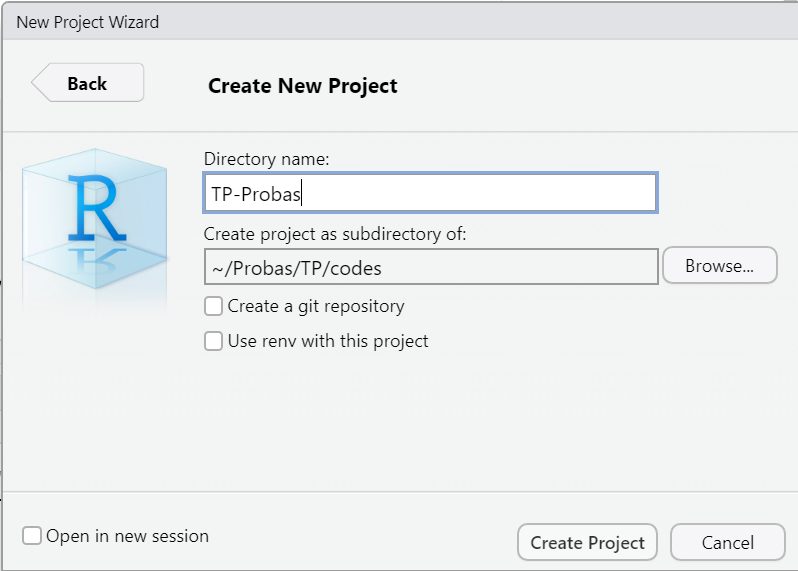
\includegraphics[width=0.5\textwidth,height=\textheight]{img/init-project-settings.png}

Un objet \texttt{R\ Project} va apparaître dans le dossier spécifié.
Placer vos fichiers avec le code initial (\texttt{generateur.R} et
\texttt{seance1.R}) dans le même dossier.

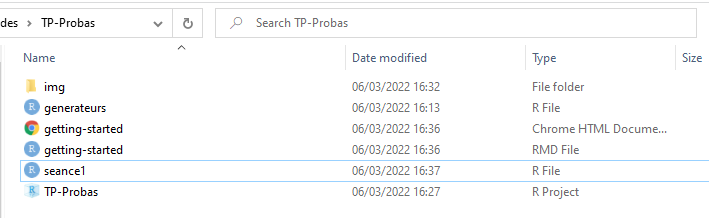
\includegraphics[width=0.5\textwidth,height=\textheight]{img/project-directory.png}

Pour le bon fonctionnement du script \texttt{seance1.R}, les deux
fichiers sources doivent être placés dans la même \emph{working
directory}.

Sur l'onglet \texttt{Files} sur le panneau droit de l'IDE
\texttt{R\ Studio}, on peut voir le contenu du chemin de travail :

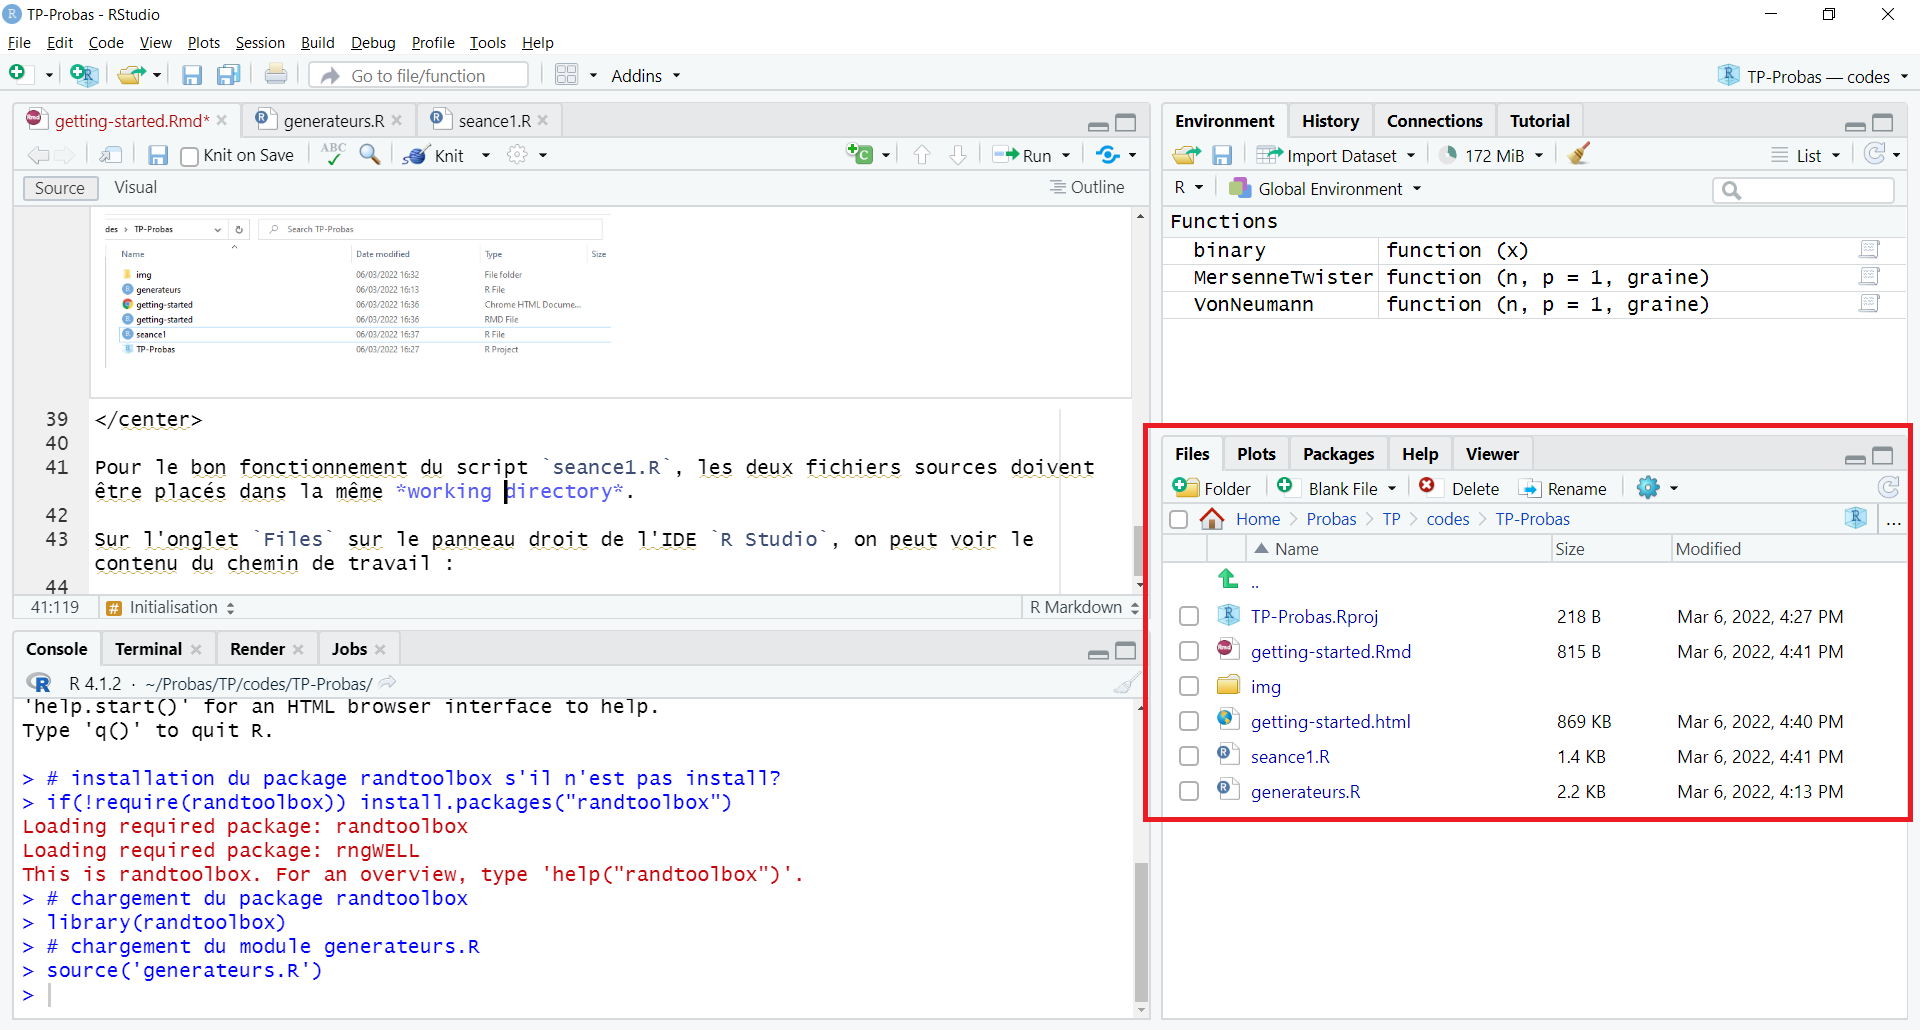
\includegraphics[width=0.75\textwidth,height=\textheight]{img/working-directory-ide.png}

\hypertarget{seance1.r}{%
\section{\texorpdfstring{\texttt{Seance1.R}}{Seance1.R}}\label{seance1.r}}

Notons qu'une fois la commande
\texttt{source(\textquotesingle{}generateurs.R\textquotesingle{})} est
exécutée, les troix fonctions définies dans \texttt{generateurs.R} sont
affichées sur l'onglet \texttt{Environment} sur le panneau droit de
l'IDE.

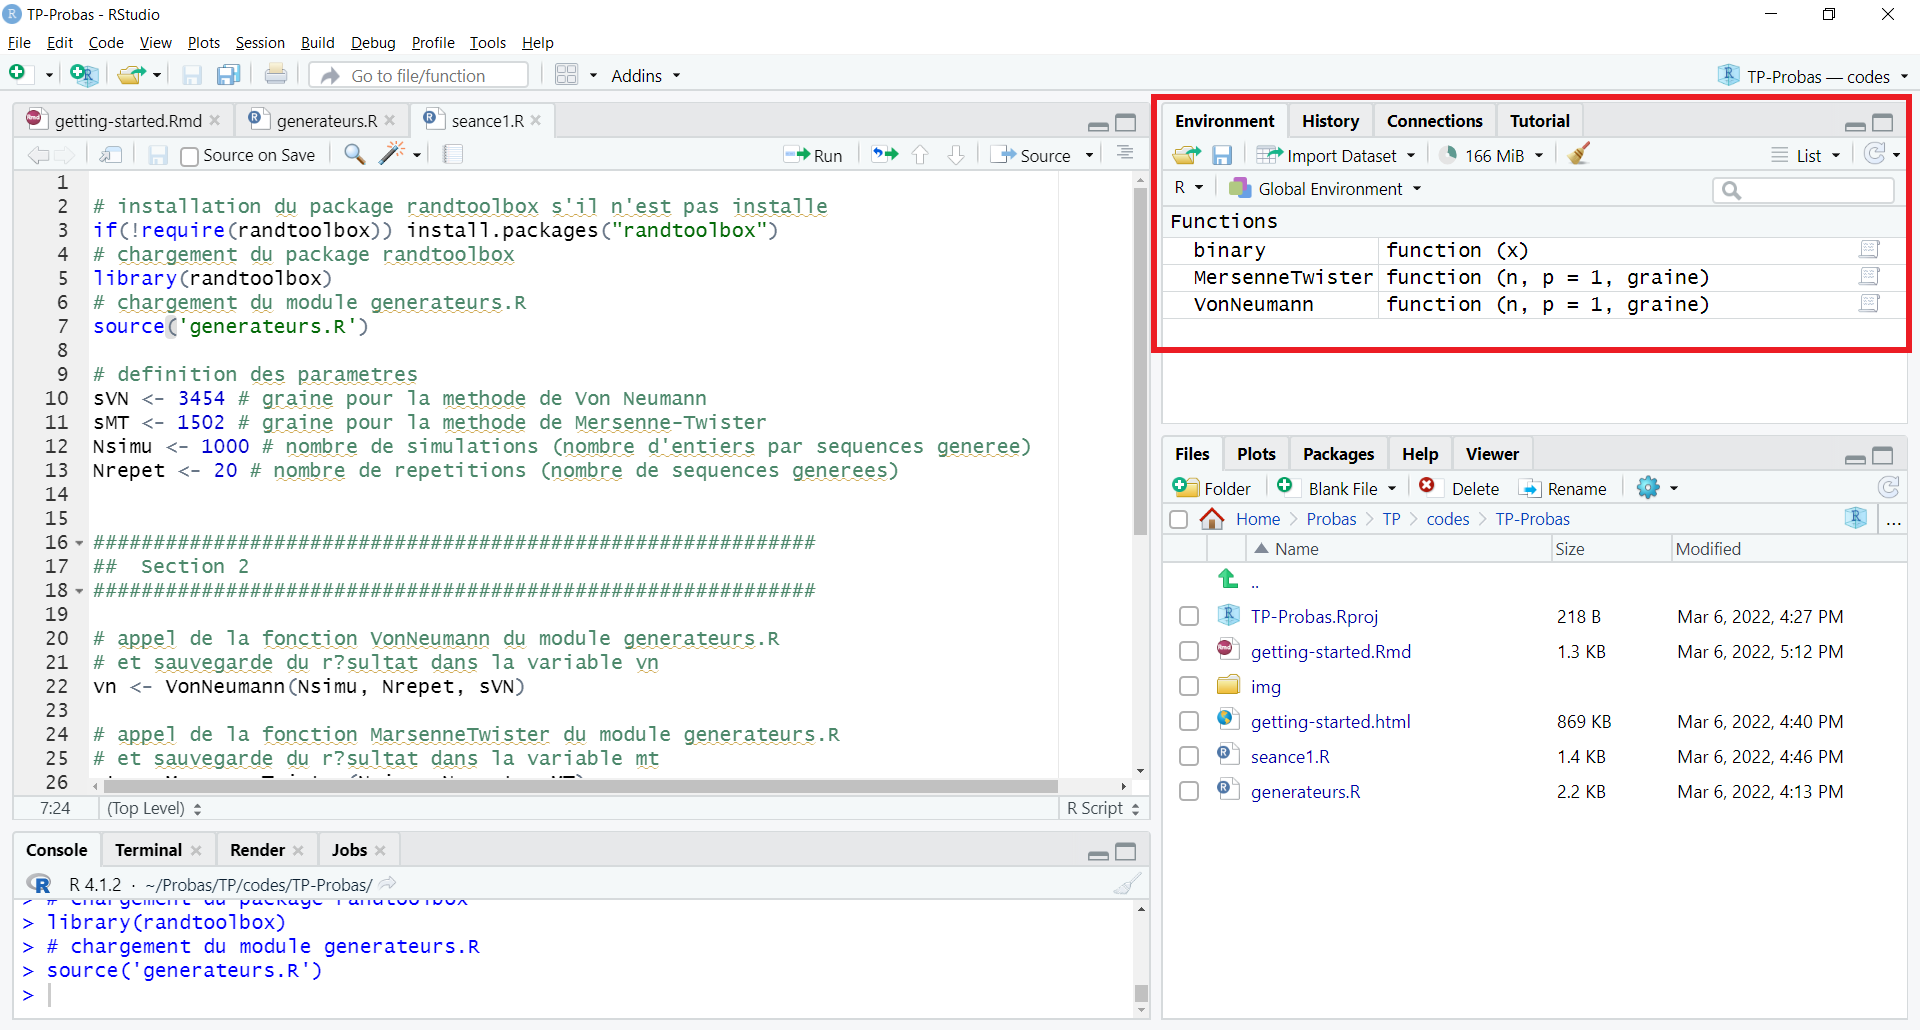
\includegraphics[width=0.75\textwidth,height=\textheight]{img/functions-tab.png}

\hypertarget{quelques-commandes-utiles}{%
\section{Quelques commandes utiles}\label{quelques-commandes-utiles}}

Pour appeler l'aide sur un objet \texttt{R} :

\begin{Shaded}
\begin{Highlighting}[]
\CommentTok{\# help}
\NormalTok{? runif }
\CommentTok{\# ou }
\FunctionTok{help}\NormalTok{(runif)}
\end{Highlighting}
\end{Shaded}

L'aide va s'ouvrir sur l'onglet \texttt{Help} sur le panneau droit de
l'IDE.

\hypertarget{vecteurs-et-matrices}{%
\subsection{Vecteurs et matrices}\label{vecteurs-et-matrices}}

\textbf{Attention ! :} le comptage (e.g.~les indices) dans le R commence
avec 1

\begin{Shaded}
\begin{Highlighting}[]
\CommentTok{\# creation d\textquotesingle{}un vecteur a l\textquotesingle{}aide de concatenation c()}
\NormalTok{x }\OtherTok{\textless{}{-}} \FunctionTok{c}\NormalTok{(}\DecValTok{1}\NormalTok{, }\DecValTok{2}\NormalTok{, }\DecValTok{3}\NormalTok{, }\DecValTok{4}\NormalTok{, }\DecValTok{5}\NormalTok{)}
\CommentTok{\# acces a un element par son indice}
\NormalTok{x[}\DecValTok{1}\NormalTok{]}
\end{Highlighting}
\end{Shaded}

\begin{verbatim}
## [1] 1
\end{verbatim}

\begin{Shaded}
\begin{Highlighting}[]
\CommentTok{\# acces aux plusieurs elements consecutifs}
\NormalTok{x[}\DecValTok{2}\SpecialCharTok{:}\DecValTok{4}\NormalTok{]}
\end{Highlighting}
\end{Shaded}

\begin{verbatim}
## [1] 2 3 4
\end{verbatim}

\begin{Shaded}
\begin{Highlighting}[]
\CommentTok{\# dans l\textquotesingle{}ordre inverse}
\FunctionTok{rev}\NormalTok{(x)}
\end{Highlighting}
\end{Shaded}

\begin{verbatim}
## [1] 5 4 3 2 1
\end{verbatim}

\begin{Shaded}
\begin{Highlighting}[]
\CommentTok{\# somme des elements du vecteur x}
\FunctionTok{sum}\NormalTok{(x)}
\end{Highlighting}
\end{Shaded}

\begin{verbatim}
## [1] 15
\end{verbatim}

\begin{Shaded}
\begin{Highlighting}[]
\CommentTok{\# incrementation de tous les elements}
\NormalTok{x }\SpecialCharTok{+} \DecValTok{2}
\end{Highlighting}
\end{Shaded}

\begin{verbatim}
## [1] 3 4 5 6 7
\end{verbatim}

\begin{Shaded}
\begin{Highlighting}[]
\CommentTok{\# multiplication des elements par une constante}
\NormalTok{x }\SpecialCharTok{*} \DecValTok{2}
\end{Highlighting}
\end{Shaded}

\begin{verbatim}
## [1]  2  4  6  8 10
\end{verbatim}

\begin{Shaded}
\begin{Highlighting}[]
\CommentTok{\# creation d\textquotesingle{}une matrice}
\NormalTok{m }\OtherTok{\textless{}{-}} \FunctionTok{matrix}\NormalTok{(}\FunctionTok{c}\NormalTok{(}\DecValTok{1}\NormalTok{,}\DecValTok{2}\NormalTok{,}\DecValTok{3}\NormalTok{,}\DecValTok{4}\NormalTok{,}\DecValTok{5}\NormalTok{,}\DecValTok{6}\NormalTok{), }\AttributeTok{nrow =} \DecValTok{3}\NormalTok{, }\AttributeTok{byrow =} \ConstantTok{TRUE}\NormalTok{); m}
\end{Highlighting}
\end{Shaded}

\begin{verbatim}
##      [,1] [,2]
## [1,]    1    2
## [2,]    3    4
## [3,]    5    6
\end{verbatim}

\begin{Shaded}
\begin{Highlighting}[]
\CommentTok{\# acces a un element par son indice}
\NormalTok{m[}\DecValTok{1}\NormalTok{,}\DecValTok{2}\NormalTok{]}
\end{Highlighting}
\end{Shaded}

\begin{verbatim}
## [1] 2
\end{verbatim}

\begin{Shaded}
\begin{Highlighting}[]
\CommentTok{\# acces a une colonne}
\NormalTok{m[,}\DecValTok{1}\NormalTok{]}
\end{Highlighting}
\end{Shaded}

\begin{verbatim}
## [1] 1 3 5
\end{verbatim}

\begin{Shaded}
\begin{Highlighting}[]
\CommentTok{\# acces a une ligne}
\NormalTok{m[}\DecValTok{2}\NormalTok{,]}
\end{Highlighting}
\end{Shaded}

\begin{verbatim}
## [1] 3 4
\end{verbatim}

\hypertarget{generation-des-suxe9quences-numuxe9riques}{%
\subsection{Generation des séquences
numériques}\label{generation-des-suxe9quences-numuxe9riques}}

\begin{Shaded}
\begin{Highlighting}[]
\CommentTok{\# sequence de nombres consécutifs}
\FunctionTok{seq}\NormalTok{(}\DecValTok{0}\NormalTok{, }\DecValTok{10}\NormalTok{)}
\end{Highlighting}
\end{Shaded}

\begin{verbatim}
##  [1]  0  1  2  3  4  5  6  7  8  9 10
\end{verbatim}

\begin{Shaded}
\begin{Highlighting}[]
\CommentTok{\# sequence de nombres consécutifs avec le pas 2}
\FunctionTok{seq}\NormalTok{(}\AttributeTok{from=}\DecValTok{0}\NormalTok{, }\AttributeTok{to=}\DecValTok{10}\NormalTok{, }\AttributeTok{by=}\DecValTok{2}\NormalTok{)}
\end{Highlighting}
\end{Shaded}

\begin{verbatim}
## [1]  0  2  4  6  8 10
\end{verbatim}

\begin{Shaded}
\begin{Highlighting}[]
\CommentTok{\# sequence de nombre consécutifs min : max (min et max y compris)}
\DecValTok{1}\SpecialCharTok{:}\DecValTok{5}
\end{Highlighting}
\end{Shaded}

\begin{verbatim}
## [1] 1 2 3 4 5
\end{verbatim}

\begin{Shaded}
\begin{Highlighting}[]
\CommentTok{\# vecteur de 5 éléments de la même valeur de 1 (répétition)}
\FunctionTok{rep}\NormalTok{(}\DecValTok{1}\NormalTok{,}\DecValTok{5}\NormalTok{)}
\end{Highlighting}
\end{Shaded}

\begin{verbatim}
## [1] 1 1 1 1 1
\end{verbatim}

\end{document}
